%*******************************************************************************
%*********************************** Fourth Chapter *****************************
%*******************************************************************************

\chapter{Quantum Measurement Backaction}  
\label{chap:backaction}
% Title of the Fourth Chapter

\ifpdf
    \graphicspath{{Chapter4/Figs/Raster/}{Chapter4/Figs/PDF/}{Chapter4/Figs/}}
\else
    \graphicspath{{Chapter4/Figs/Vector/}{Chapter4/Figs/}}
\fi


%********************************** %First Section  **************************************

\section{Introduction}

This thesis is entirely concerned with the question of measuring a
quantum many-body system using quantized light. However, so far we
have only looked at expectation values in a nondestructive context
where we neglect the effect of the quantum wavefunction collapse. We
have shown that light provides information about various statistical
quantities of the quantum states of the atoms such as their
correlation functions. In general, any quantum measurement affects the
system even if it doesn't physically destroy it. In our model both
optical and matter fields are quantized and their interaction leads to
entanglement between the two subsystems. When a photon is detected and
the electromagnetic wavefunction of the optical field collapses, the
matter state is also affected due to this entanglement resulting in
quantum measurement backaction. Therefore, in order to determine these
quantities multiple measurements have to be performed to establish a
precise measurement of the expectation value which will require
repeated preparations of the initial state.

In the following chapters, we consider a different approach to quantum
measurement in open systems and instead of considering expectation
values we look at a single experimental run and the resulting dynamics
due to measurement backaction. Previously, we were mostly interested
in extracting information about the quantum state of the atoms from
the scattered light. The flexibility in the measurement model was used
to enable probing of as many different quantum properties of the
ultracold gas as possible. By focusing on measurement backaction we
instead investigate the effect of photodetections on the dynamics of
the many-body gas as well as the possible quantum states that we can
prepare instead of what information can be extracted.

In this chapter, we introduce the necessary theory of quantum
measurement and backaction in open systems in order to lay a
foundation for the material that follows in which we apply these
concepts to a bosonic quantum gas. We first introduce the concept of
quantum trajectories which represent a single continuous series of
photon detections. We also present an alternative approach to open
systems in which the measurement outcomes are discarded. This will be
useful when trying to learn about dynamical features common to every
trajectory. In this case we use the density matrix formalism which
obeys the master equation. This approach is more common in dissipative
systems and we will highlight the differences between these two
different types of open systems. We conclude this chapter with a new
concept that will be central to all subsequent discussions. In our
model measurement is global, it couples to operators that correspond
to global properties of the quantum gas rather than single-site
quantities. This enables the possibility of performing measurements
that cannot distinguish certain sites from each other. Due to a lack
of ``which-way'' information this leads to the creation of spatially
nontrivial virtual lattices on top of the physical lattice. This turns
out to have significant consequences on the dynamics of the system.

\section{Quantum Trajectories}

A simple intuitive concept of a quantum trajectory is that it is the
path taken by a quantum state over time during a single experimental
realisation. In particular, we consider states conditioned upon
measurement results such as the photodetection times. Such a
trajectory is generally stochastic in nature as light scattering is
not a deterministic process. Furthermore, they are in general
discotinuous as each detection event brings about a drastic change in
the quantum state due to the wavefunction collapse of the light field.

Before we discuss specifics relevant to our model of quantized light
interacting with a quantum gas we present a more general overview
which will be useful as some of the results in the following chapters
are more general. Measurement always consists of at least two
competing processes, two possible outcomes. If there is no competition
and only one outcome is possible then our probe is meaningless as it
does not reveal any information about the system. In its simplest form
measurement consists of a series of detection events, such as the
detections of photons. Even though, on an intuitive level it seems
that we have defined only a single outcome, the detection event, this
arrangement actually consists of two mutually exclusive outcomes. At
any point in time an event either happens or it does not, a photon is
either detected or the detector remains silent, also known as a null
result. Both outcomes reveal some information about the system we are
investigating. For example, let us consider measuring the number of
atoms by measuring the number of photons they scatter. Each atom will
on average scatter a certain number of photons contributing to the
detection rate we observe. Therefore, if we record multiple photons at
a high rate of arrival we learn that the illuminated region must
contain many atoms. On the other hand, if there are few atoms to
scatter the light we will observe few detection events which we
interpret as a continuous series of non-detection events interspersed
with the occasional detector click. This trajectory informs us that
there are much fewer atoms being illuminated than previously.

Basic quantum mechanics tells us that such measurements will in
general affect the quantum state in some way. Each event will cause a
discontinuous quantum jump in the wavefunction of the system and it
will have a jump operator, $\c$, associated with it. The effect of a
detection event on the quantum state is simply the result of applying
this jump operator to the wavefunction, $| \psi (t) \rangle$,
\begin{equation}
  \label{eq:jump}
  | \psi(t + \mathrm{d}t) \rangle = \frac{\c | \psi(t) \rangle}
  {\sqrt{\langle \cd \c \rangle (t)}},
\end{equation}
where the denominator is simply a normalising factor
\cite{MeasurementControl}. The exact form of the jump operator $\c$
will depend on the nature of the measurement we are considering. For
example, if we consider measuring the photons escaping from a leaky
cavity then $\c = \sqrt{2 \kappa} \hat{a}$, where $\kappa$ is the
cavity decay rate and $\hat{a}$ is the annihilation operator of a
photon in the cavity field. It is interesting to note that due to
renormalisation the effect of a single quantum jump is independent of
the magnitude of the operator $\c$ itself. However, larger operators
lead to more frequent events and thus more frequent applications of
the jump operator.

The null measurement outcome will have an opposing effect to the
quantum jump, but it has to be treated differently as it does not
occur at discrete time points like the detection events themselves
\cite{MeasurementControl}. Its effect is accounted for by a
modification to the isolated Hamiltonian, $\hat{H}_0$, time evolution
in the form
\begin{equation}
  | \psi (t + \mathrm{d}t) \rangle = \left\{ \hat{1} - \mathrm{d}t
    \left[ i \hat{H}_0 + \frac{\cd \c}{2} - \frac{\langle \cd \c
        \rangle (t)}{2} \right] \right\} | \psi (t) \rangle.
\end{equation}
The effect of both outcomes can be included in a single stochastic
Schr\"{o}dinger equation given by
\begin{equation}
  \label{eq:SSE}
  \mathrm{d} | \psi(t) \rangle = \left[ \mathrm{d} N(t) \left(
      \frac{\c} {\sqrt{ \langle \cd \c \rangle (t)}} - \hat{1} \right)
    + \mathrm{d} t \left( \frac{\langle \cd \c \rangle (t)}{2} -
      \frac{ \cd \c}{2} - i \hat{H}_0 \right) \right] | \psi(t) \rangle,
\end{equation}
where $\mathrm{d}N(t)$ is the stochastic increment to the number of
photodetections up to time $t$ which is equal to $1$ whenever a
quantum jump occurs and $0$ otherwise \cite{MeasurementControl}. Note
that this equation has a straightforward generalisation to multiple
jump operators, but we do not consider this possibility here at all.

All trajectories that we calculate in the follwing chapters are
described by the stochastic Schr\"{o}dinger equation in
Eq. \eqref{eq:SSE}. The most straightforward way to solve it is to
replace the differentials by small time-steps $\delta t$. Then we
generate a random number $R(t)$ at every time-step and a jump is
applied, i.e.~$\mathrm{d}N(t) = 1$, if
\begin{equation}
  R(t) < \langle \cd \c \rangle (t) \delta t.
\end{equation}

In practice, this is not the most efficient method for simulation
\cite{MeasurementControl}. Instead we will use the following
method. At an initial time $t = t_0$ a random number $R$ is
generated. We then propagate the unnormalised wavefunction
$| \tilde{\psi} (t) \rangle$ using the non-Hermitian evolution given
by
\begin{equation}
  \frac{\mathrm{d}}{\mathrm{d}t} | \tilde{\psi} (t) \rangle = -i
  \left( \hat{H}_0 - i \frac{\cd \c}{2} \right) | \tilde{\psi} (t) \rangle
\end{equation}
up to a time $T$ such that
$\langle \tilde{\psi} (T) | \tilde{\psi} (T) \rangle = R$. This
problem can be solved efficienlty using standard numerical
techniques. At time $T$ a quantum jump is applied according to
Eq. \eqref{eq:jump} which renormalises the wavefunction as well and
the process is repeated as long as desired. This formulation also has
the advantage that it provides a more intuitive picture of what
happens during a single trajectory. The quantum jumps are
self-explanatory, but now we have a clearer picture of the effect of
null outcomes on the quantum state. Its effect is entirely encoded in
the non-Hermitian modification to the original Hamiltonian given by
$\hat{H} = \hat{H}_0 - i \cd \c / 2$. It is now easy to see that for a
jump operator, $\c$, with a large magnitude the no-event outcomes will
have a more significant effect on the quantum state. At the same time
they will lead to more frequent quantum jumps which have an opposing
effect to the non-Hermitian evolution, because the jump condition is
satisfied $\langle \tilde{\psi} (T) | \tilde{\psi} (T) \rangle = R$
more frequently. In general, the competition between these two
processes is balanced and without any further external influence the
distribution of outcomes over many trajectories will be entirely
determined by the initial state even though each individual trajectory
will be unique and conditioned on the exact detection times that
occured during the given experimental run. However, individual
trajectories can have features that are not present after averaging
and this is why we focus our attention on single experimental runs
rather than average behaviour.

\begin{figure}[htbp!]
  \centering
  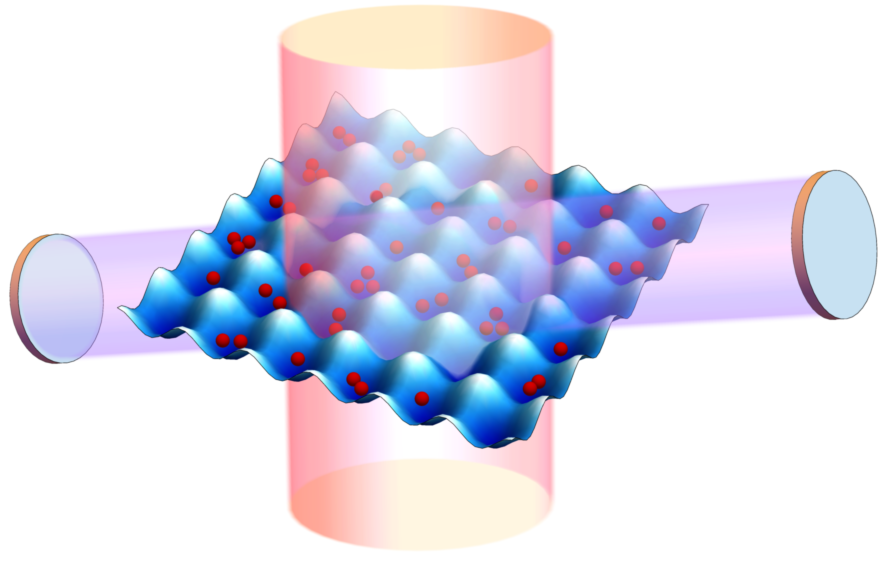
\includegraphics[width=1.0\textwidth]{setup}
  \caption[Experimental Setup with Cavity]{Atoms in an optical lattice
    are probed by a coherent light beam (red), and the light scattered
    (blue) at a particular angle is enhanced and collected by a leaky
    cavity. The photons escaping the cavity are detected, perturbing
    the atomic evolution via measurement backaction.}
  \label{fig:cavity}
\end{figure}

The quantum trajectory theory can now be very straightforwardly
applied to our model of ultracold bosons in an optical
lattice. However, from now on we will only consider the case when the
atomic system is coupled to a single mode cavity in order to enhance
light scattering in one particular direction as shown in
Fig. \ref{fig:cavity}. This way we have complete control over the form
of the quantum jump operator, because light scattering in different
directions corresponds to different measurements as we have seen in
Eq. \eqref{eq:Jcoeff}. On the other hand, in free space we would have
to simultaneously consider all the possible directions in which light
could scatter and thus include multiple jump operators reducing our
ability to control the system.

The model we derived in Eq. \eqref{eq:fullH} is in fact already in a
form ready for quantum trajectory simulations. The phenomologically
included cavity decay rate $-i \kappa \ad_1 \a_1$ is in fact the
non-Hermitian term $-i \cd \c / 2$, where $\c = \sqrt{2 \kappa} \a_1$
which is the jump operator we want for measurements of photons leaking
from the cavity. However, we will first simplify the system by
considering the regime where we can neglect the effect of the quantum
potential that builds up in the cavity. Physically, this means that
whilst light scatters due to its interaction with matter, the field
that builds up due to the scattered photons collecting in the cavity
has a negligible effect on the atomic evolution compared to its own
dynamics such as inter-site tunnelling or on-site interactions. This
can be achieved when the cavity-probe detuning is smaller than the
cavity decay rate, $\Delta_p \ll \kappa$
\cite{caballero2015}. However, even though the cavity field has a
negligible effect on the atoms, measurement backaction will not. This
effect is of a different nature. It is due to the wavefunction
collapse due to the destruction of photons rather than an interaction
between fields. Therefore, the final form of the Hamiltonian
Eq. \eqref{eq:fullH} that we will be using in the following chapters
is
\begin{equation}
  \label{eq:backaction}
  \hat{H} = \hat{H}_0 - i \gamma \hat{F}^\dagger \hat{F}
\end{equation}
\begin{equation}
  \hat{H}_0 = -J \sum_{\langle i, j \rangle} \bd_i b_j + \frac{U}{2}
                \sum_i \n_i (\n_i - 1),
\end{equation}
where $\hat{H}_0$ is simply the Bose-Hubbard Hamiltonian,
$\gamma = \kappa |C|^2$ is a quantity that measures the strength of
the measurement and we have substituted $\a_1 = C \hat{F}$. The
quantum jumps are applied at times determined by the algorithm
described above and the jump operator is given by
\begin{equation}
  \label{eq:jumpop}
  \c = \sqrt{2 \kappa} C \hat{F}.
\end{equation}
Importantly, we see that measurement introduces a new energy and time
scale $\gamma$ which competes with the two other standard scales
responsible for the unitary dynamics of the closed system, tunnelling,
$J$, and on-site interaction, $U$.  If each atom scattered light
inependently a different jump operator $\c_i$ would be required for
each site projecting the atomic system into a state where long-range
coherence is degraded. This is a typical scenario for spontaneous
emission \cite{pichler2010, sarkar2014}, or for local
\cite{syassen2008, kepesidis2012, vidanovic2014, bernier2014,
  daley2014} and fixed-range addressing \cite{ates2012, everest2014}
which are typically considered in open systems. In contrast to such
situations, we consider global coherent scattering with an operator
$\c$ that is nonlocal. Therefore, the effect of measurement backaction
is global as well and each jump affects the quantum state in a highly
nonlocal way and most importantly not only will it not degrade
long-range coherence, it will in fact lead to such long-range
correlations itself.

In Chapter \ref{chap:qnd} we used highly efficient DMRG methods
\cite{tnt} to calculate the ground state of the Bose-Hubbard
Hamiltonian. Related techniques such as Time-Evolving Block Decimation
(TEBD) or t-DMRG are often used for numerical calculations of time
evolution. However, despite the fact our Hamiltonian in
Eq. \eqref{eq:backaction} is simply the Bose-Hubbard model with a
non-Hermitian term added due to measurement it is actually difficult
to apply these methods to our system. The problem lies in the fact
that Matrix Product methods we mentioned are only efficient for
one-dimensional systems that obey the area law for entanglement
entropy, i.e.~systems with only short-range quantum
correlations. Unfortunately, the global nature of the measurement we
consider violates the assumptions made in deriving the area law and,
as we shall see in the following chapters, leads to long-range
correlations regardless of coupling strength. Therefore, we resort to
using exact methods such as exact diagonalisation which we solve with
well-known ordinary differential equation solvers. This means that we
can at most simulate a few atoms, but as we shall see it is the
geometry of the measurement that matters the most and these effects
are already visible in smaller systems.

\section{The Master Equation}
\label{sec:master}

A quantum trajectory is stochastic in nature, it depends on the exact
timings of the quantum jumps which are determined randomly. This makes
it difficult to obtain conclusive deterministic answers about the
behaviour of single trajectories. One possible approach that is very
common when dealing with open systems is to look at the unconditioned
state which is obtained by averaging over the random measurement
results which condition the system \cite{MeasurementControl}. The
unconditioned state is no longer a pure state and thus must be
described by a density matrix,
\begin{equation}
  \label{eq:rho}
  \hat{\rho} = \sum_i p_i | \psi_i \rangle \langle \psi_i |,
\end{equation}
where $p_i$ is the probability the system is in the pure state
$| \psi_i \rangle$. If more than one $p_i$ value is non-zero then the
state is mixed, it cannot be represented by a single pure state. The
time evolution of the density operator obeys the master equation given
by
\begin{equation}
  \dot{\hat{\rho}} = -i \left[ \hat{H}_0, \hat{\rho} \right] + \c
  \hat{\rho} \cd - \frac{1}{2} \left( \cd \c \hat{\rho} + \hat{\rho}
    \cd \c \right).
\end{equation}
Physically, the unconditioned state, $\rho$, represents our knowledge
of the quantum system if we are ignorant of the measurement outcome
(or we choose to ignore it), i.e.~we do not know the timings of the
detection events. 

We will be using the master equation and the density operator
formalism in the context of measurement. However, the exact same
methods are also applied to a different class of open systems, namely
dissipative systems \cite{QuantumNoise}. A dissipative system is an
open system that couples to an external bath in an uncontrolled
way. The behaviour of such a system is similar to a system subject
under observation in which we ignore all the results. One can even
think of this external coupling as a measurement who's outcome record
is not accessible and thus must be represented as an average over all
possible trajectories. However, there is a crucial difference between
measurement and dissipation. When we perform a measurement we use the
master equation to describe system evolution if we ignore the
measuremt outcomes, but at any time we can look at the detection times
and obtain a conditioned pure state for this current experimental
run. On the other hand, for a dissipative system we simply have no
such record of results and thus the density matrix predicted by the
master equation, which in general will be a mixed state, represents
our best knowledge of the system. In order to obtain a pure state, it
would be necessary to perform an actual measurement.

A definite advantage of using the master equation for measurement is
that it includes the effect of any possible measurement
outcome. Therefore, it is useful when extracting features that are
common to many trajectories, regardless of the exact timing of the
events. However, in this case we do not want to impose any specific
trajectory on the system as we are not interested in a specific
experimental run, but we would still like to identify the set of
possible outcomes and their common properties. Unfortunately,
calculating the inverse of Eq. \eqref{eq:rho} is not an easy task. In
fact, the decomposition of a density matrix into pure states might not
even be unique. However, if a measurement leads to a projection,
i.e.~the final state becomes confined to some subspace of the Hilbert
space, then this will be visible in the final state of the density
matrix. We will show this on an example of a qubit in the quantum
state
\begin{equation}
  \label{eq:qubit0}
  | \psi \rangle = \alpha |0 \rangle + \beta | 1 \rangle,
\end{equation}
where $| 0 \rangle$ and $| 1 \rangle$ represent the two basis states
of the qubit and we consider performing a measurement in the basis
$\{| 0 \rangle, | 1 \rangle \}$, but we don't check the outcome.  The
quantum state will have collapsed now to the state $ | 0 \rangle$ with
probability $| \alpha |^2$ and $| 1 \rangle$ with probability
$| \beta |^2$. The corresponding density matrix is given by
\begin{equation}
  \label{eq:rho1}
  \hat{\rho} = \left( \begin{array}{cc}
                        | \alpha |^2 & 0 \\
                        0 & |\beta|^2 
                      \end{array} \right),
\end{equation}
which is a mixed state as opposed to the initial state. We note that
there are no off-diagonal terms as the system is not in a
superposition between the two basis states. Therefore, the diagonal
terms represent classical probabilities of the system being in either
of the basis states. This is in contrast to their original
interpretation when the state was given by Eq. \eqref{eq:qubit0} when
they could not be interpreted as in such a way. The initial state was
in a quantum superposition and thus the state was indeterminate due to
the quantum uncertainty in our knowledge of the state which would have
manifested itself in the density matrix as non-zero off-diagonal
terms. The significance of these values being classical probabilities
is that now we know that the measurement has already happened and we
know with certainty that the state must be either $| 0 \rangle$ or
$| 1 \rangle$. We just don't know which one until we check the result
of the measurement.

We have assumed that it was a discrete wavefunction collapse that lead
to the state in Eq. \eqref{eq:rho1} in which case the conclusion we
reached was obvious. However, the nature of the process that takes us
from the initial state to the final state with classical uncertainty
does not matter. The key observation is that regardless of the
trajectory taken, if the final state is given by Eq. \eqref{eq:rho1}
we will definitely know that our state is either in the state
$| 0 \rangle$ or $| 1 \rangle$ and not in some superposition of the
two basis states. Therefore, if we obtained this density matrix as a
result of applying the time evolution given by the master equation we
would be able to identify the final states of individual trajectories
even though we have no information about the individual trajectories
themself. This is analogous to an approach in which decoherence due to
coupling to the environment is used to model the wavefunction collapse
\cite{zurek2002}, but here we will be looking at projective effects
due to weak measurement.

Here we have considered a very simple case of a Hilbert space with two
non-degenerate basis states. In the following chapters we will
generalise the above result to larger Hilbert spaces with multiple
degenerate subspaces which are of much greater interest as they reveal
nontrivial dynamics in the system.

\section{Global Measurement and ``Which-Way'' Information}
\label{sec:modes}

We have already mentioned that one of the key features of our model is
the global nature of the measurement operators. A single light mode
couples to multiple lattice sites from where atoms scatter the light
coherently into a single mode which we enhance and collect with a
cavity. If atoms at different lattice sites scatter light with a
different phase or magnitude we will be able to identify which atoms
contributed to the light we detected. However, if they scatter the
photons in phase and with the same amplitude then we have no way of
knowing which atom emitted the photon, we have no ``which-way''
information. When we were considering nondestructive measurements and
looking at expectation values, this had no consequence on our results
as we were simply interested in probing the quantum correlations of a
given ground state and whether two sites were distinguishable or not
was irrelevant. Now, on the other hand, we are interested in the
effect of these measurements on the dynamics of the system. The effect
of measurement backaction will depend on the information that is
encoded in the detected photon. If a scattered mode cannot
distinuguish between two different lattice sites then we have no
information about the distribution of atoms between those two sites.
Therefore, all quantum correlations between the atoms in these sites
are unaffected by the backaction whilst their correlations with the
rest of the system will change as the result of the quantum jumps.

\begin{figure}[htbp!]
  \centering
  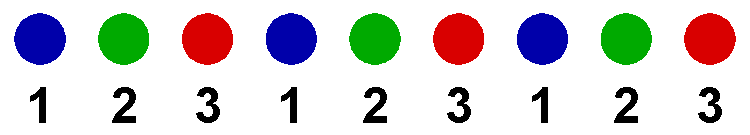
\includegraphics[width=1.0\textwidth]{1DModes}
  \caption[1D Modes due to Measurement Backaction]{The coefficients,
    and thus the operator $\hat{D}$ is made periodic with a period of
    three lattice sites. Therefore, the coefficients $J_{i,i}$ will
    repeat every third site making atoms in those sites
    indistinguishable to the measurement. Physically, this is due to
    the fact that this periodic arrangement causes the atoms within a
    single mode to scatter light with the same phase and amplitude.
    The scattered light contains no information which can be used to
    determine the atom distribution.}
  \label{fig:1dmodes}
\end{figure}

The quantum jump operator for our model is given by
$\c = \sqrt{2 \kappa} C \hat{F}$ and we know from Eq. \eqref{eq:F}
that we have a large amount of flexibility in tuning $\hat{F}$ via the
geometry of the optical setup. A cavity aligned at a different angle
will correspond to a different measurement. We will consider the case
when $\hat{F} = \hat{D}$ given by Eq. \eqref{eq:D}, but since the
argument depends on geometry rather than the exact nature of the
operator it straightforwardly generalises to other measurement
operators, including the case when $\hat{F} = \hat{B}$ where the bonds
(inter-site operators) play the role of lattice sites. The operator
$\hat{D}$ is given by
\begin{equation}
  \hat{D} = \sum_i J_{i,i} \n_i,
\end{equation}
where the coefficients $J_{i,i}$ are determined from
Eq. \eqref{eq:Jcoeff}. These coefficients represent the coupling
strength between the atoms and the light modes and thus their spatial
variation can be easily tuned by the geometry of the optical
fields. We are in particular interested in making these coefficients
degenerate across a number of lattice sites as shown in
Figs. \ref{fig:1dmodes} and \ref{fig:2dmodes}. Note that they do not
have to be periodic, but it is much easier to make them so. This makes
all lattice sites with the same value of $J_{i,i}$ indistinguishable
to the measurement thus partitioning the lattice into a number of
distinct zones which we will refer to as modes. It is crucial to note
that these partitions in general are not neighbours of each other,
they are not localised, they overlap in a nontrivial way, and the
patterns can be made more complex in higher dimensions as shown in
Fig. \ref{fig:2dmodes} or with a more sophisticated optical setup
\cite{caballero2016}. This has profound consquences as it can lead to
the creation of long-range nonlocal correlations between lattice sites
\cite{mazzucchi2016, kozlowski2016zeno}. The measurement does not know
which atom within a certain mode scattered the light, there is no
``which-way'' information. Therefore, from the point of view of the
observer's knowledge all atoms within a mode are identical regardless
of their spatial separation. This effect can be used to create virtual
lattices on top of the physical lattice.

\begin{figure}[htbp!]
  \centering
  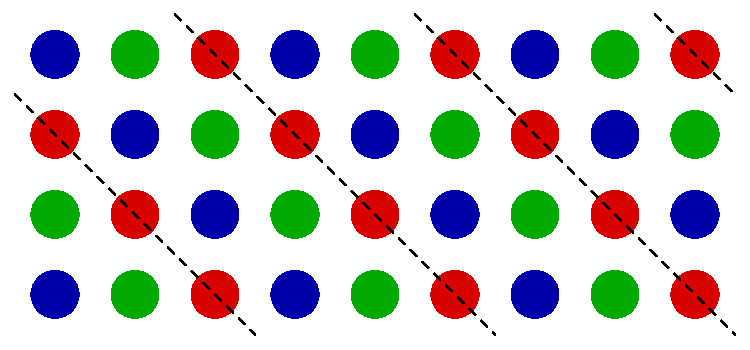
\includegraphics[width=1.0\textwidth]{2DModes}
  \caption[2D Modes due to Measurement Backaction]{ More complex
    patterns of virtual lattice can be created in higher
    dimensions. With a more complicated setup even more complicated
    geometries are possible.}
  \label{fig:2dmodes}
\end{figure}

We will now look at a few practical examples.  The simplest case is to
measure in the diffraction maximum such that $\a_1 = C \hat{N}_K$,
where $\hat{N}_K = \sum_j^K \hat{n}_j$ is the number of atoms in the
illuminated area. If the whole lattice is illuminated we effectively
have a single mode as $J_{i,i} = 1$ for all sites. If only a subset of
lattice sites is illuminated $K < M$ then we have two modes
corresponding to the illuminated and unilluminated sites. It is
actually possible to perform such a measurement in a nonlocal way by
arranging every other site (e.g.~all the even sites) to be at a node
of both the cavity and the probe. The resulting field measures the
number of atoms in the remaining sites (all the odd sites) in a global
manner. It does not know how these atoms are distributed among these
sites as we do not have access to the individual sites. This two mode
arrangement is shown in the top panel of Fig. \ref{fig:twomodes}. A
different two-mode arrangement is possible by measuring in the
diffraction minimum such that each site scatters in anti-phase with
its neighbours as shown in the bottom panel of
Fig. \ref{fig:twomodes}. 

\begin{figure}[htbp!]
  \centering
  
\includegraphics[width=0.7\textwidth]{TwoModes1}
  
\includegraphics[width=0.7\textwidth]{TwoModes2}
  \caption[Two Mode Partitioning]{Top: only the odd sites scatter
    light leading to a measurement of $\hat{N}_\mathrm{odd}$ and an
    effectove partitiong into even and odd sites. Bottom: this also
    partitions the lattice into odd and even sites, but this time
    atoms at all sites scatter light, but in anti-phase with their
    neighbours.}
  \label{fig:twomodes}
\end{figure}

This can approach can be generalised to an arbitrary number of modes,
$Z$. For this we will conisder a deep lattice such that
$J_{i,i} = u_1^* (\b{r}) u_0 (\b{r})$. We will take the probe beam to
be incident normally at a 1D lattice so that $u_0 (\b{r}) =
1$. Therefore, the final form of the scattered light field is given by
\begin{equation}
  \label{eq:Dmodes}
  \a_1 = C \hat{D} = C \sum_m^K \exp\left[-i k_1 m d \sin \theta_1
  \right] \hat{n}_m.
\end{equation}
From this equation we see that it can be made periodic with a period
$Z$ when
\begin{equation}
  k_1 d \sin \theta_1 = 2\pi R / Z,
\end{equation}
where $R$ is just some integer and $R/Z$ are is a fraction in its
simplest form. Therefore, we can rewrite the Eq. \eqref{eq:Dmodes} as
a sum of the indistinguishable contributions from the $Z$ modes
\begin{equation}
  \label{eq:Zmodes}
  \a_1 = C \hat{D} = C \sum_l^Z \exp\left[-i 2 \pi l R / Z \right] \hat{N}_l,
\end{equation}
where $\hat{N}_l = \sum_{m \in l} \n_m$ is the sum of single site atom
number operators that belong to the same mode. $\hat{N}_K$ and
$\hat{N}_\mathrm{odd}$ are the simplest examples of these modes. This
partitions the 1D lattice in exactly $Z > 1$ modes by making every
$Z$th lattice site scatter light with exactly the same phase. It is
interesting to note that these angles correspond to the $K-1$
classical diffraction minima.

